\documentclass[
  bibliography=totoc,     % Literatur im Inhaltsverzeichnis
  captions=tableheading,  % Tabellenüberschriften
  titlepage=firstiscover, % Titelseite ist Deckblatt
]{scrartcl}

% Paket float verbessern
\usepackage{scrhack}

% Warnung, falls nochmal kompiliert werden muss
\usepackage[aux]{rerunfilecheck}

% unverzichtbare Mathe-Befehle
\usepackage{amsmath}
% viele Mathe-Symbole
\usepackage{amssymb}
% Erweiterungen für amsmath
\usepackage{mathtools}

% Fonteinstellungen
\usepackage{fontspec}
% Latin Modern Fonts werden automatisch geladen
% Alternativ zum Beispiel:
%\setromanfont{Libertinus Serif}
%\setsansfont{Libertinus Sans}
%\setmonofont{Libertinus Mono}

% Wenn man andere Schriftarten gesetzt hat,
% sollte man das Seiten-Layout neu berechnen lassen
\recalctypearea{}

% deutsche Spracheinstellungen
\usepackage{polyglossia}
\setmainlanguage{german}


\usepackage[
  math-style=ISO,    % ┐
  bold-style=ISO,    % │
  sans-style=italic, % │ ISO-Standard folgen
  nabla=upright,     % │
  partial=upright,   % ┘
  warnings-off={           % ┐
    mathtools-colon,       % │ unnötige Warnungen ausschalten
    mathtools-overbracket, % │
  },                       % ┘
]{unicode-math}

% traditionelle Fonts für Mathematik
\setmathfont{Latin Modern Math}
% Alternativ zum Beispiel:
%\setmathfont{Libertinus Math}

\setmathfont{XITS Math}[range={scr, bfscr}]
\setmathfont{XITS Math}[range={cal, bfcal}, StylisticSet=1]

% Zahlen und Einheiten
\usepackage[
  locale=DE,                   % deutsche Einstellungen
  separate-uncertainty=true,   % immer Fehler mit \pm
  per-mode=symbol-or-fraction, % / in inline math, fraction in display math
]{siunitx}

% chemische Formeln
\usepackage[
  version=4,
  math-greek=default, % ┐ mit unicode-math zusammenarbeiten
  text-greek=default, % ┘
]{mhchem}

% richtige Anführungszeichen
\usepackage[autostyle]{csquotes}

% schöne Brüche im Text
\usepackage{xfrac}

% Standardplatzierung für Floats einstellen
\usepackage{float}
\floatplacement{figure}{htbp}
\floatplacement{table}{htbp}

% Floats innerhalb einer Section halten
\usepackage[
  section, % Floats innerhalb der Section halten
  below,   % unterhalb der Section aber auf der selben Seite ist ok
]{placeins}

% Seite drehen für breite Tabellen: landscape Umgebung
\usepackage{pdflscape}

% Captions schöner machen.
\usepackage[
  labelfont=bf,        % Tabelle x: Abbildung y: ist jetzt fett
  font=small,          % Schrift etwas kleiner als Dokument
  width=0.9\textwidth, % maximale Breite einer Caption schmaler
]{caption}
% subfigure, subtable, subref
\usepackage{subcaption}

% Grafiken können eingebunden werden
\usepackage{graphicx}
% größere Variation von Dateinamen möglich
\usepackage{grffile}

% schöne Tabellen
\usepackage{booktabs}

% Verbesserungen am Schriftbild
\usepackage{microtype}

% Literaturverzeichnis
\usepackage[
  backend=biber,
]{biblatex}
% Quellendatenbank
\addbibresource{lit.bib}
\addbibresource{programme.bib}

% Hyperlinks im Dokument
\usepackage[
  unicode,        % Unicode in PDF-Attributen erlauben
  pdfusetitle,    % Titel, Autoren und Datum als PDF-Attribute
  pdfcreator={},  % ┐ PDF-Attribute säubern
  pdfproducer={}, % ┘
]{hyperref}
% erweiterte Bookmarks im PDF
\usepackage{bookmark}

% Trennung von Wörtern mit Strichen
\usepackage[shortcuts]{extdash}

\author{%
  AUTOR A\\%
  \href{mailto:authorA@udo.edu}{authorA@udo.edu}%
  \texorpdfstring{\and}{,}%
  AUTOR B\\%
  \href{mailto:authorB@udo.edu}{authorB@udo.edu}%
}
\publishers{TU Dortmund – Fakultät Physik}


\begin{document}
%1
\maketitle
%2
\begin{frame}{\huge{List of Contents}}
  \begin{columns}
    \column{.5\textwidth}
      \begin{itemize}
        \setlength\itemsep{1em}
        \item About me
        \item Proton Imaging
        \item Motivation for the Bachelor Thesis
        \item Experimental Setup
        \item FE-I4 Module
        \item What's next?
      \end{itemize}
    \column{.5\textwidth}
      \begin{figure}
        \centering
        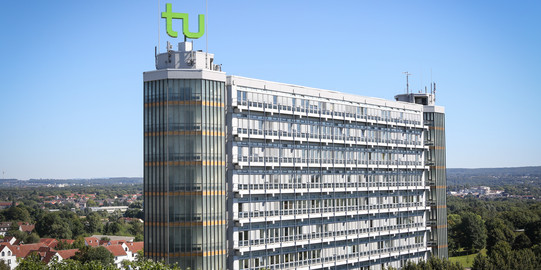
\includegraphics[width=\textwidth]{figures/tu.jpg}
      \end{figure}
\end{columns}
\end{frame}

%3
\begin{frame}{\huge{About me}}
  \begin{itemize}
    \setlength\itemsep{1em}
    \item Name: Felix Gläsemann
    \item Age: 27
    \item Intended degree: Bachelor in medical physics
    \item Hobbies:
      \begin{itemize}
        \item[\rightarrow] Running, swimming
        \item[\rightarrow] Reading
        \item[\rightarrow] Going out with friends
      \end{itemize}
  \end{itemize}
\end{frame}
%4
\begin{frame}{\huge{Proton Imaging}}
  \begin{columns}
    \column{.6\textwidth}
    \begin{itemize}
      \setlength\itemsep{1em}
      \item Proton beams to create images of tissue
        \begin{itemize}
          \item[\rightarrow] Protons interact with tissue
          \item[\rightarrow] Signals from the interaction get detected
          \item[\rightarrow] Images are reconstructed
        \end{itemize}
        \item Advantages:
        \begin{itemize}
          \item[\rightarrow] Reduced radiation dose
        \end{itemize}
        \item Application in medical imaging and materials science
      \end{itemize}
      \column{.4\textwidth}
        \begin{figure}
          \centering
          \label{fig:rpr}
          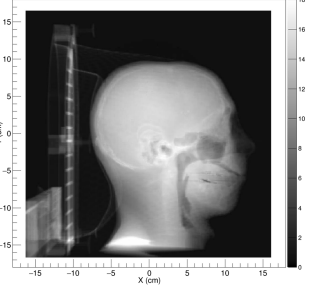
\includegraphics[width=.9\textwidth]{figures/pi.png}
          \caption*{Reconstructed proton radiograph (RPR) \cite[p.~99]{pi}}
        \end{figure}
    \end{columns}
\end{frame}
%5
\begin{frame}{\huge{Motivation for the Bachelor Thesis}}
  \begin{columns}[t]
    \column{.6\textwidth}
    \begin{itemize}
      \item Physical and medical application
      \begin{itemize}
        \item[\rightarrow] Improving diagnostics through \textbf{proton imaging} and \textbf{therapy}
        \item[\rightarrow] Better understanding of proton detection for different tunings of the detector
        \item[\rightarrow] Influence of tuning on clustering and measured charge
      \end{itemize}
    \end{itemize}
    \column{.4\textwidth}
  \begin{figure}
    \label{fig:pixde}
    \centering
    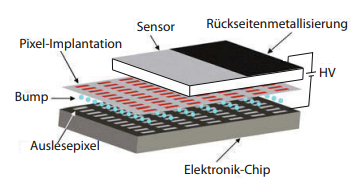
\includegraphics[width=.9\textwidth]{figures/detektor.png}
    \caption*{Schematic structure of a pixelated silicon detector \cite[p.~334]{kola}}
  \end{figure}
\end{columns}
\end{frame}
%6
\begin{frame}{\huge{Motivation for the Bachelor Thesis}}
  \begin{itemize}
    \item Comparison between experiment and simulation
  \end{itemize}
\begin{figure}
  \label{fig:landau}
  \centering
  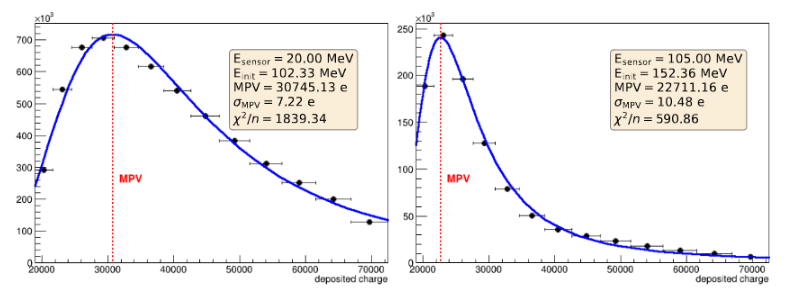
\includegraphics[width=.9\textwidth]{figures/landau_comp.png}
\end{figure}
\end{frame}
%7
\begin{frame}{\huge{Experimental Setup}}
  \begin{figure}
    \centering
    \label{fig:exset}
    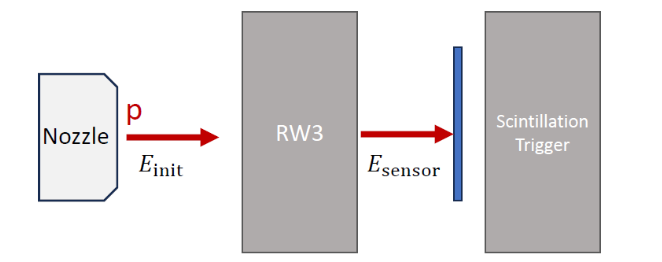
\includegraphics[scale=.4]{figures/exset.png}
  \end{figure}
  \begin{itemize}
    \item RW3 phantom used to lower the energy of the protons
    \item FE-I4 used for detection
  \end{itemize}
\end{frame}
%8
\begin{frame}
\frametitle{\huge{FE-I4 Module}}
  \begin{columns}
    \column{.4\textwidth}
    \begin{itemize}
      \item FE-I4
      \begin{itemize}
        \item[\rightarrow] Developed for ATLAS Experiment
        \item[\rightarrow] High-speed data readout
        \item[\rightarrow] Identify and process relevant data from particle collisions
      \end{itemize}
    \end{itemize}
    \column{.6\textwidth}
    \begin{figure}
      \centering
      \label{fig:exset2}
      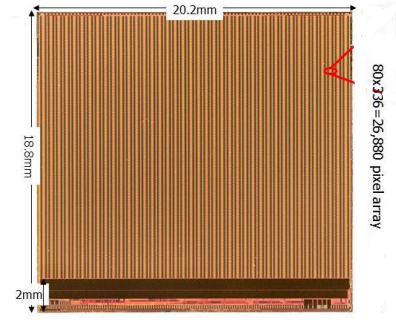
\includegraphics[scale=.6]{figures/exset2.png}
      \caption*{FE-I4 module \cite[p.~3]{exset2}}
    \end{figure}
  \end{columns}
\end{frame}
%9
\begin{frame}{\huge{What's next?}}
  \begin{itemize}
    \setlength\itemsep{1em}
    \item Building the experimental setup using Allpix Squared
    \item Start the simulation and get first results
    \begin{itemize}
      \item[\rightarrow] Compare results from experiment and simulation
    \end{itemize}
  \end{itemize}
\end{frame}
%9
\begin{frame}
  \centering \Huge\textcolor{tugreen}{\textbf{Questions?}}
\end{frame}

\appendix
\begin{frame}[t]
\frametitle{\huge{Literature}}
\printbibliography{}
\end{frame}
\end{document}
